\documentclass[tikz, margin=5mm]{standalone}
\usepackage[sfdefault,light]{roboto}
\usetikzlibrary{shapes, arrows, positioning, fit, backgrounds}
\definecolor{MyGreen}{HTML}{41B3A3}
\definecolor{MyOrange}{HTML}{E27D60}
\tikzset{every picture/.style={/utils/exec={\sffamily}}}
\begin{document}
    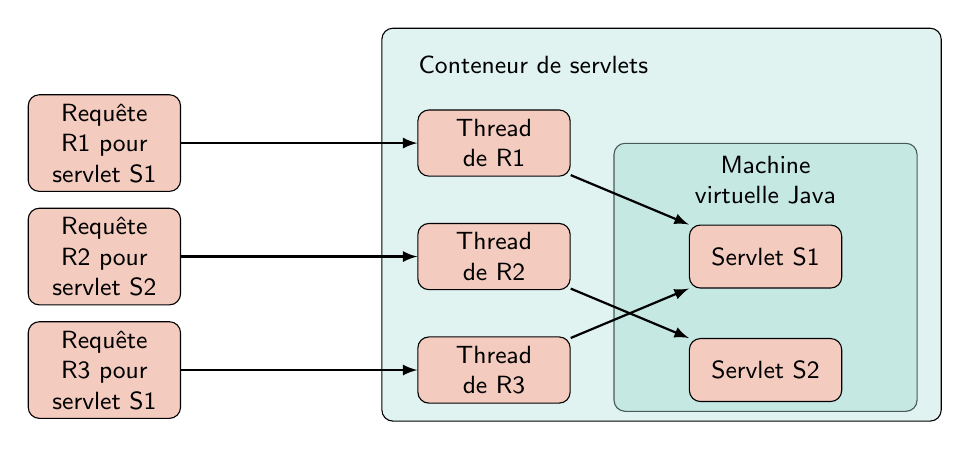
\begin{tikzpicture}	[
			every node/.style={font=\small, align=center, draw, fill=MyOrange!40, rectangle, rounded corners, minimum height=8mm, text width=17mm},
			server/.style={draw, fill=MyGreen!40}
		]
			\node (client1) [] {Requête R1 pour servlet S1};
			\node (client2) [below=0.2cm of client1] {Requête R2 pour servlet S2};
			\node (client3) [below=0.2cm of client2] {Requête R3 pour servlet S1};	
			
			\node (thread1) [right=3cm of client1] {Thread de R1};
			\node (thread2) [right=3cm of client2] {Thread de R2};
			\node (thread3) [right=3cm of client3] {Thread de R3};
			
			\node (serv1) [right=1.5cm of thread2] {Servlet S1};
			\node (serv2) [right=1.5cm of thread3] {Servlet S2};
			
			\node (JVMLegend) [above right=1mm and 5mm of thread1.north, anchor=south, draw=none, fill=none, text height=1mm, text width=30mm] {Conteneur de servlets};
			\node (ContainerLegend) [above=1mm of serv1.north, anchor=south, draw=none, fill=none, text height=1mm, text width=30mm] {Machine virtuelle Java};
			
			
			\begin{scope}[on background layer]
				\node (container) [
					server, fill opacity=.6, inner xsep=3mm,
					fit={(serv1) (serv2) (ContainerLegend)}
				] {};
				\node (server) [
					server, inner xsep=3mm, fill opacity=.4,
					fit={(thread1) (thread2) (thread3) (container) (JVMLegend)}
				] {};
			\end{scope}

			\draw[-latex,thick] (client1) -- (thread1);
			\draw[-latex,thick] (thread1) -- (serv1);
			\draw[-latex,thick] (client2) -- (thread2);
			\draw[-latex,thick] (thread2) -- (serv2);
			\draw[-latex,thick] (client3) -- (thread3);
			\draw[-latex,thick] (thread3) -- (serv1);
		\end{tikzpicture}
\end{document}